\documentclass{standalone}
\usepackage{tikz}
\begin{document}
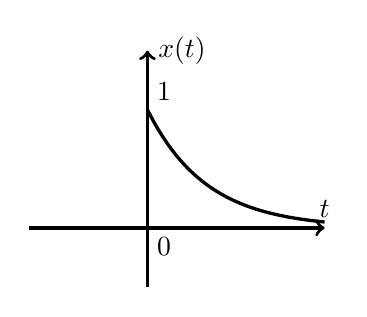
\begin{tikzpicture}[scale=1.5]
    \draw[->,very thick](-1,0)--(1.5,0)node[above]{$t$};
        \draw[->,very thick](0,-0.5)--(0,1.5)node[right]{$x(t)$};
        \node[below right]at(0,0){$0$};
        \node[above right]at(0,1){$1$};

        \draw[-,very thick](-1,0)--(0,0);
        \draw[-,very thick]plot[smooth, domain=0:1.5](\x,{e^(-2*(\x))});
\end{tikzpicture}
\end{document}